\chapter{Topologie sur le corps des complexes}
\section{Les structures d'espace vectoriel normé sur le corps des complexes}

L'ensemble $\C$ des nom\-bres complexes possède deux structures naturelles d'espace vectoriel, l'une d'espace vectoriel complexe et l'autre d'espace vectoriel réel. 
\begin{fprop}
$\C$ agissant sur lui-même par produit est un espace vectoriel de dimension 1. Un endomorphisme $f$ de $\C$ est une application de la forme:
\[
f \colon z \in \C \mapsto \lambda z
\]
avec $\lambda \in \C$.
\end{fprop}
\begin{proof}
$\C$ muni de son addition usuelle est un groupe abélien. L'action par produit de $\C$ sur lui-même vérifie pour tout quadruplet $(u,v,z_0,z_1)$ de complexes:
\[
u.(z_1 + z_0) = u.z_1 + u.z_0, \, (u+v).z = u.z+ v.z, \, (uv).z = u.(v.z), \, 1. z = z
\]
Il s'agit donc d'un espace vectoriel. Pour tout complexe $z$, on a de façon évidente $z = z . 1$, montrant que le complexe $1$ est une base de $\C$.

Si $f$ est un endomorphisme de $\C$, on a pour tout complexe $z$:
\[
f(z) = f(z.1)=z.f(1)
\]
qui correspond à la forme annoncée avec $\lambda = f(1)$.
\end{proof}
\begin{fprop}
\label{prop:corps_matrices}
L'ensemble des matrices de la forme:
\[
\left(
\begin{array}{cc}
a   &  -b \\
b     & a
\end{array}
\right)
\]
est un corps commutatif, isomorphe au corps des complexes.
\end{fprop}
\begin{proof}
Les matrices de la forme donnée sont inversibles si et seulement si $a^2+b^2 \neq 0$ et sont stables par addition et produit. L'élément neutre pour la multiplication est la matrice identité, l'élément neutre pour l'addition la matrice nulle.
L'isomorphisme est donné par:
\[
\phi \colon 
\begin{pmatrix}
x   &  -y \\
y     & x
\end{pmatrix} \mapsto x + i y
\]
Un calcul élémentaire montre que que l'on a:
\[
\phi(MN) = \phi(M).\phi(N)
\]
\end{proof}
\begin{fprop}
\label{prop:r2_c}
Le groupe additif $\R^2$ muni de l'action par produit du corps de la proposition \ref{prop:corps_matrices} est un espace vectoriel de dimension 1, isomorphe à l'espace vectoriel complexe $\C$.
\end{fprop}
\begin{proof}
Tout point $(x,y)$ de $\R^2$ est un multiple du vecteur de base $(1,0)$:
\[
\begin{pmatrix}
x \\
y
\end{pmatrix} = 
\begin{pmatrix}
x & -y \\
y & x 
\end{pmatrix}
\begin{pmatrix}
1 \\0
\end{pmatrix}
\]
montrant ainsi que l'espace vectoriel est de dimension 1. 
L'isomorphisme avec $\C$ est: $\psi \colon (x,y) \mapsto x + i y$ (on vérifiera sans peine qu'il s'agit d'une application linéaire).
\end{proof}
La propriété ci-dessous est élémentaire, mais fondamentale.
\begin{fprop}
L'application  $z \in \C \mapsto |z|=\sqrt{z \overline{z}}$ est une norme sur l'espace vectoriel complexe $\C$.
\end{fprop}
\begin{rem}
Le module est ce que l'on appelle une valeur absolue, à  avoir une application $| \cdot |$ définie sur un corps $K$, à valeurs dans $\R^+$ et vérifiant les trois axiomes suivants:
\[
\begin{split}
&|x| = 0 \Leftrightarrow x = 0 \textit{ (séparation) }\\
&|x+y| \leq |x| + |y|, \, x,y  \in K \textit{ (inégalité triangulaire) }\\
& |xy| = |x||y|, \, x,y \in K \textit{ (produit) }
\end{split}
\]
Sur le corps de la proposition \ref{prop:corps_matrices}, l'application $M \mapsto |M| = \det{M}^{1/2}$ est une valeur absolue qui est compatible avec l'isomorphisme $\phi$: $|M| = |\phi(M)|$.
\end{rem}
L'espace vectoriel réel $\R^2$ est de dimension 2, une base en étant par exemple $e_1=(1,0), e_2 = (0,1)$. De même, $\C$ est un espace vectoriel réel de dimension 2 en prenant comme base $(1,i)$. Il existe un isomorphisme canonique entre ces espaces vectoriels donné par $(x,y) \mapsto x + i y$. Tout endormorphisme de l'espace vectoriel réel $\R^2$ est de la forme:
\[
f \colon \begin{pmatrix}
x \\ y
\end{pmatrix}  \mapsto \begin{pmatrix}
a & b \\
c & d 
\end{pmatrix}\begin{pmatrix}
x \\ y
\end{pmatrix}
\]
Il se transporte sur $\C$ par l' isomorphisme canonique:
\[
f \colon (x+iy) \mapsto ax + by + i \left(cx + dy\right)
\]
En remarquant que $x = (z+\overline{z})/2, y = (z - \overline{z})/(2i)$, on peut obtenir une écriture plus facile à interpréter:
\[
f \colon z \mapsto \left((a+d)+i(c-b)\right)\frac{z}{2} + \left((a-d)+i(b+c)\right)\frac{\overline{z}}{2}
\]
On remarque dans l'expression précédente que le premier terme est un endomorphisme de $\C$ (en tant que $\C$ espace vectoriel) alors que le second est $\C$-antilinéaire, selon la définition ci-dessous.
\begin{fdefn}
Une application $f \colon \mathbb{C} \to \mathbb{C}$ est dite $\mathbb{C}$-antilinéaire, si pour tout triplet $(\lambda,z_1,z_2) \in \mathbb{C}^3$, on a $f(z_1 + z_2) = f(z_1)+f(z_2)$ et $f(\lambda z)= \overline{\lambda} f(z)$.
\end{fdefn}
Toute application $\R$-linéaire sur $\C$ se décompose donc de façon unique comme somme d'un endomorphisme de $\C$ et d'une application $\C$-antilinéaire. La proposition suivante est un corollaire immédiat de cette remarque.
\begin{fprop}
\label{prop:endomorphisme_c}
Soit $f$ un endomorphisme de $\R^2$ de matrice associée:
\[
\begin{pmatrix}
a & b \\
c & d
\end{pmatrix}
\]
Il est transporté en un endomorphisme de $\C$ par l' isomorphisme canonique si et seulement si $a=d,b=-c$.
\end{fprop}
\begin{rem}
On retrouve sans surprise le corps des matrices de la proposition \ref{prop:r2_c}. Le cas des applications $\C$-antilinéaires est cependant très différent car les matrices correspondantes sont de la forme:
\[
\begin{pmatrix}
a & b \\
b & -a
\end{pmatrix}
\]
et ne constituent pas un corps, n'étant pas stables par produit. La structure algébrique correspondante sort du cadre de ce cours. 
\end{rem}

\section{Topologie}
\subsection{Parties ouvertes, parties fermées}
Les différentes notions de topologie présentées ici sont celles utilisées dans la suite du cours. Les énoncés se font dans le cadre particulier de $\C$, mais s'appliquent à tous les espaces vectoriels normés de dimension finie. 
\begin{fdefn}
	Un disque ouvert du plan complexe, centré en $z_0$ et de rayon $r$, est la partie de $\C$ définie par~:
	\[D(z_0,r) = \{ z \in \C , \lvert z-z_0 \rvert <r\}.\]
\end{fdefn}
\begin{rem}
 Le terme de disque ouvert est réservé aux espaces vectoriels normés de dimension deux. Dans le cas général, on parlera de boule ouverte, qui se définit de façon identique en remplaçant le module par la norme dans la définition précédente.
 \end{rem}
\begin{fdefn}
	Soit $z$ un point de $\C$. Une partie $V$ de $\C$ sera appelée un \textbf{voisinage} de $z$ si il existe un disque ouvert $D(z,r), r > 0$ contenu dans $V$.
\end{fdefn}
Les voisinages sont les briques de base de la topologie. Ils permettent en particulier de définir la notion de convergence d'une suite ou de continuité d'une fonction.
\begin{fdefn}
    \textbf{Convergence d'une suite :}
	Soit $(z_n), n  \in \N$ une suite de points de $\C$. On dira qu'elle converge vers une limite $z_\infty$ si pour tout voisinage $V$ de $z_\infty$, il existe un entier $N_V$ tel que:
	\[
	\forall n \geq N_V, z_n \in V
	\]
\end{fdefn}
Dans le cas de $\C$ et de façon générale pour tous les espaces métriques, il est possible de se limiter aux disques ouverts (boules ouvertes en dimension quelconque). Une suite $z_n, n \in \N$ convergera vers une limite $z_\infty$ si et seulement si pour tout réel strictement positif $\epsilon$, il existe un entier $N_\epsilon$  tel que:
\[
\forall n \geq N_\epsilon, \,|z_n-z_\infty| < \epsilon
\]
\begin{fdefn}
\textbf{Continuité :}
Soit $A$ une partie de $\C$ et soit $f$ une application $f \colon A \to \C$. On dira que $f$ est continue au point $z_0$ de $A$ si pour tout voisinage $V$ de $f(z_0)$, il existe un voisinage $W$ de $z_0$ tel que $f\left(W \cap A\right) \subset V$.
\end{fdefn}
Ici encore il est possible de se limiter à des voisinages qui sont des disques ouverts. On notera que la définition précédente ne suppose rien sur la partie $A$.
\begin{fdefn} Un sous ensemble $U$ du plan complexe est appelé un \textbf{ouvert} si il est voisinage de chacun de ses points. 
\end{fdefn}
En d'autres termes, si $U$ est un ouvert, alors, pour tout point $z$ de $U$, il existe un disque ouvert $D(z,r),r>0$ contenu dans $U$. L'ensemble des ouverts de $\C$, noté $\mathcal{O}(\C)$ est appelé topologie de $\C$.

\begin{prop}
Un disque ouvert $D(z_0,r)$ est un ouvert. 
\end{prop}
\begin{proof}
	Soit $z$ un élément de $D(z_0,r)$. Le disque $D(z,r-|z-z_0|)$ est contenu dans $D(z_0,r)$ car si $u$ est l'un de ses points, on a:
	\[
	|u-z_0| \leq |u-z| + |z-z_0| < r - |z-z_0| + |z-z_0| = r
	\]
	$D(z_0,r)$ est donc un voisinage de chacun de ses points. 
\end{proof}

\begin{defn}
Le disque fermé de centre $z_0$ et de rayon $r$ est la partie du plan complexe définie par :
\[
\overline{D}(z_0,r) = \{ z  \in \C , |z-z_0| \leq r  \}
\]
\end{defn}

\begin{fprop}
	Un disque fermé n'est pas un ouvert.
\end{fprop}
\begin{proof}
	Soit $z$ tel que $|z-z_0| = r$. Pour tout $\epsilon > 0$, le point $\eta = z + \frac{\epsilon}{2r}(z-z_0)$ appartient à $D(z,\epsilon)$ car $|\eta - z| = \epsilon / 2 < \epsilon$ mais n'appartient pas à $\overline{D}(z_0,r)$ car $|\eta - z_0| = r+\epsilon/2 > r$.
\end{proof}
\begin{fprop}
	Les propriétés suivantes sont vérifiées par les ouverts:
	\begin{itemize}
		\item $\emptyset,\C$ sont des ouverts.
		\item Pour toute famille finie $U_i, i=1\dots n$ d'ouverts, $\bigcap_{i=1}^n U_i$ est un ouvert.
		\item Pour toute famille $U_i, i \in I$ d'ouverts, $\bigcup_{i \in I}U_i$ est un ouvert.
	\end{itemize}
\end{fprop}
\begin{rem}
	En topologie générale, les propriétés précédentes servent à définir les ouverts. 
\end{rem}
\begin{fprop}
	Pour toute partie $A$ de $\C$ il existe un plus grand ouvert contenu dans $A$, appelé intérieur de $A$ et noté $\mathring{A}$.
\end{fprop}
\begin{proof}
	L'ensemble des ouverts contenus dans $A$ n'est pas vide car $\emptyset$ lui appartient. La réunion de tous les ouverts contenus dans $A$ est donc bien définie et est encore un ouvert. C'est le plus grand, au sens de l'inclusion, de tous les ouverts inclus dans $A$.
\end{proof}
\begin{fdefn}
	Un fermé est le complémentaire d'un ouvert.
\end{fdefn}
La proposition suivante est une conséquence immédiate de la définition des fermés.
\begin{fprop}
	Les propriétés suivantes sont vérifiées par les fermés:
	\begin{itemize}
		\item $\emptyset,\C$ sont des fermés.
		\item Pour toute famille finie $F_i, i=1\dots n$ de fermés, $\bigcup_{i=1}^n F_i$ est un fermé.
		\item Pour toute famille $F_i, i \in I$ de fermés, $\bigcap_{i \in I}F_i$ est un fermé.
	\end{itemize}
\end{fprop}
La proposition suivante est similaire à celle concernant l'intérieur d'une partie. 
\begin{fprop}
	Pour toute partie $A$ de $\C$, il existe un plus petit fermé contenant $A$, appelé adhérence de $A$ et noté $\overline{A}$.
\end{fprop}
\begin{fdefn}
	La frontière d'une partie $A$ est le fermé: $\partial A = \overline{A}-\mathring{A}$. 
\end{fdefn}
\begin{prop}
	Un disque fermé $\overline{D}(z_0,r)$ est un fermé.
\end{prop}
\begin{proof}
	Il suffit de montrer que son complémentaire est un ouvert. Soit $z$ un point de $\C$ tel que $|z-z_0|>r$. Le disque ouvert $D(z,r-|z-z_0|)$ est contenu dans le complémentaire de $\overline{D}(z_0,r)$ car si $|u-z| < r - |z -z_0|$, on a:
	\[
	|u-z_0| > \left | \strut |z-z_0| - |u-z| \right | > r -r + |z-z_0| > r
	\]
	Le complémentaire de  $\overline{D}(z_0,r)$ est un voisinage de chacun de ses points, donc est un ouvert.
\end{proof}

La proposition suivante se révèle souvent utile pour démontrer qu'un ensemble est fermé :
\begin{fprop}
	Soit $F$ une partie fermée de $\C$. Soit $(z_n), n \in \N$ une suite de points de $F$ convergeant vers une limite $z_\infty$. Alors $z_\infty \in F$.
\end{fprop}
\begin{proof}
	Supposons que $z_\infty \notin F$. $F^c$ étant ouvert, il existe un disque ouvert $D(z,r), r> 0$ contenu dans $F^c$. Ce disque est un voisinage de $z_\infty$ et ne contient aucun terme de la suite $(z_n), n \in \N$, ce qui est une contradiction avec la définition de la limite. 
\end{proof}
\subsection{Suites de Cauchy et complétude}
La détermination de la limite d'une suite est souvent difficile. Dans certains espaces topologiques, il existe néanmoins un critère simple permettant d'affirmer qu'une suite converge.

\begin{prop}
Une suite $(z_n), n \in \N$ de nombres complexes converge si et seulement si les suites réelles $\operatorname{Re} (z_n)_n$ et $\operatorname{Im} (z_n)_n$ convergent.
\end{prop}
\begin{fdefn}
	Soit $(z_n),n \in N$ une suite de nombres complexes. On dira qu'elle est de Cauchy si:
	\[
	\forall \epsilon > 0, \, \exists N_\epsilon \in \N, \, \forall m,n \geq N_\epsilon, |z_m-z_n| < \epsilon
	\]
\end{fdefn}
On notera que toute suite de Cauchy est bornée, car à partir d'un certain rang, tous les termes de la suite appartiennent à une boule de rayon fini arbitraire. 
\begin{fprop}
	Toute suite convergente est de Cauchy.
\end{fprop}
\begin{proof}
	Soit $(z_n),n\in \N$ une suite de limite $z_\infty$. Pour tout $\epsilon > 0$, il existe $N_\epsilon$ tel que si $n \geq N_\epsilon$, $|z_n - z_\infty| < \epsilon / 2$. Par l'inégalité triangulaire on a donc:
	\[
	\forall m,n \geq N_\epsilon, |z_n -z_m| \leq |z_n - z_\infty| + |z_m - z_\infty| < \epsilon
	\]
	La suite est donc de Cauchy.
\end{proof}
La réciproque est en général fausse, mais lorsqu'elle est vraie, on dit que l'espace est complet. C'est le cas de $\R$ lorsqu'il est muni de la topologie induite par la valeur absolue. 

Avant de donner la preuve de cette propriété, il convient de rappeler que dans $\R$, toute partie $A$ non vide majorée possède une borne supérieure, notée $\sup(A)$ (il s'agit d'un des axiomes définissant $\R$). On peut en donner une caractérisation simple.
\begin{fprop}
Soit $A$ une partie non vide majorée de $\R$. Sa borne supérieure $\sup(A)$ est l'unique majorant de $A$ vérifiant:
\[
\forall \epsilon > 0, \exists a \in A \lvert a > \sup(A) - \epsilon
\]
\end{fprop}
\begin{proof}
On rappelle que la borne supérieure d'une partie majorée est le plus petit élément de l'ensemble des majorants. Pour tout $\epsilon > 0$, $\sup(A)-\epsilon < \sup(A)$ et il existe donc $a \in A$ tel que $a > \sup(A) - \epsilon$. Réciproquement, soit $m$ est un majorant de $A$ vérifiant:
\[
\forall \epsilon > 0, \exists a \in A \lvert a > m - \epsilon
\]
Pour tout majorant $M$ de $A$ et tout $\epsilon > 0$, on a $m-\epsilon < M$ et par passage à la limite: $m \leq M$. $m$ est donc le plus petit élément de l'ensemble des majorants.
\end{proof}
On définira de même la borne inférieure d'une partie minorée $A$ que l'on notera $\inf(A)$. 
Une conséquence immédiate de cette caractérisation de la borne supérieure est la proposition suivante.
\begin{fprop}
Toute suite réelle $(x_n)_{n \in \N}$ croissante et majorée converge. De même, toute suite décroissante et minorée converge.
\end{fprop}
\begin{proof}
Il suffit de montrer la première partie de la proposition, la seconde s'en déduisant immédiatement.
Soit $l = \sup \{ x_n, n \in \N \}$. Pour tout $\epsilon > 0$, il existe un entier $N_\epsilon$ tel que $x_{N_\epsilon} > l - \epsilon$. La suite étant croissante, pour tout $n \geq N_\epsilon$, $x_n \in ]l-\epsilon, l+\epsilon[$, prouvant que $(x_n)_{n \in \N}$ est convergente de limite $l$.
\end{proof}
\begin{fprop}
Soit $(x_n)_{n \in N}$ une suite réelle bornée. Soient les réels $\limsup_n  x_n, \liminf_n x_n$ définis par:
\[
\begin{cases}
\limsup_n x_n = \lim \{ \sup \{ x_k, k \geq n \}, n \in \N\} = \inf \{ \sup \{ x_k, k \geq n \}, n \in \N\} \\
\liminf_n x_n = \lim \{ \inf \{ x_k, k \geq n \}, n \in \N\} = \sup \{ \inf \{ x_k, k \geq n \}, n \in \N\} \\
\end{cases}
\]
La suite $(x_n)_{n \in N}$ est convergente si et seulement si $\limsup_n  x_n =  \liminf_n x_n$
\end{fprop}
\begin{proof}
On remarquera tout d'abord que $\limsup_n  x_n, \liminf_n x_n$ sont bien définis car bornes supérieures ou inférieures de parties bornées. Si la suite $(x_n)_{n \in N}$ est convergente de limite $l$, pour tout $\epsilon > 0$, il existe un entier $N_\epsilon$ tel que pour tout $n \geq N_\epsilon$, $x_n \in ]l-\epsilon, l+ \epsilon[$. On en déduit que $\limsup_n x_n < l+ \epsilon$ et $\liminf_n x_n > l- \epsilon$ et, en faisant tendre $\epsilon$ vers 0, que $\limsup_n x_n = \liminf_n x_n= l$. Réciproquement, si $\limsup_n x_n = \liminf_n x_n= l$, pour tout $\epsilon > 0$ il existera un rang $N_\epsilon$ à partir duquel $x_n$ sera dans l'intervalle $]l-\epsilon, l+\epsilon[$, prouvant que la suite est convergente. 
\end{proof}
\begin{fprop}
$\R$ est un espace complet.
\end{fprop}
\begin{proof}
Soit $(x_n)_{n \in \N}$ une suite de Cauchy. Elle est donc bornée et les réels:  $\limsup_n  x_n, \liminf_n x_n$ sont bien définis.
 Pour tout $\epsilon > 0$, il existe un entier $N_\epsilon$ tel que pour tout couple $(m,n)$ d'entiers supérieurs
  à $N_\epsilon$, $|x_n-x_m| < \epsilon$. Par définition des limites supérieures et inférieures, 
  il existe également un entier $M_\epsilon$ (resp. $P_\epsilon$) tel que $x_p > \liminf_n x_n - \epsilon, p \geq M_\epsilon$ (resp. $x_q < \limsup_n x_n +  \epsilon, q \geq P_\epsilon$). Soit $p,q$ deux entiers supérieurs à $\sup \{ N_\epsilon, M_\epsilon, P_\epsilon\}$. Par l'inégalité triangulaire il vient:
\[
\left |\limsup_n x_n - \liminf_n x_n \right | \leq 
\left| \limsup_n x_n - x_p\right | + \left| x_p - x_q\right | + 
\left| \liminf_n x_n - x_q\right |  < 3 \epsilon
\]
En faisant tendre $\epsilon$ vers 0, on a donc:
\[
\limsup_n x_n = \liminf_n x_n 
\]
prouvant ainsi que la suite est convergente. 
\end{proof}
\begin{fprop}
	$\C$ est un espace complet.
\end{fprop}
\begin{proof}
	La preuve est élémentaire lorsque l'on admet que $\R$ est un espace complet. Soit $(z_n)_{n \in \N}$ une suite de Cauchy dans $\C$. On pose $z_n = x_n + i y_n$ avec $(x_n)_{n \in \N},(y_n)_{n \in \N}$ suites réelles. Soit $\epsilon > 0$. Il existe un entier $N_\epsilon$ tel que pour tout couple d'entiers $n,m$ supérieurs à $N_\epsilon$:
	\[
	\sqrt{(x_m-x_n)^2+(y_m-y_n)^2} < \epsilon
	\]
	d'où l'on tire:
	\[
	|x_m-x_n|<\epsilon, \, |y_m-y_n| < \epsilon
	\]
	Ceci montre que les suites $(x_n)_{n \in \N},(y_n)_{n \in \N}$ sont elles-mêmes de Cauchy donc convergentes dans $\R$ complet. Soient $x_\infty,y_\infty$ leurs limites respectives et $z_\infty=x_\infty+iy_\infty$. Par l'inégalité triangulaire:
	\[
	|z_n - z_\infty| \leq |x_n - x_\infty|+|y_n-y_\infty|
	\]
	Ceci montre que $(z_n)_{n \in \N}$ est convergente, de limite $z_\infty$.
\end{proof}
\begin{rem}
On remarquera que la démonstration précédente s'applique à tout espace vectoriel réel de dimension finie.
\end{rem}
\subsection{Compacité}
La notion de partie compacte est particulièrement importante en topologie, et intervient dans de nombreux théorèmes. 
\begin{fdefn}
	On dit qu'une partie $A$ de $\C$ est compacte si pour toute famille d'ouverts $U_i, i \in I$ telle que $A \subset \bigcup_{i\in I} U_i $, il existe une sous-famille finie $U_{i_j}, j=1\dots n$ telle que $A \subset\bigcup_{j=1\dots n} U_{i_j}$. De façon équivalente en passant aux complémentaires, $A$ sera une partie compacte si pour toute famille de fermés $F_i, i \in I$ telle que $\bigcap_{i\in I} F_i \bigcap A= \emptyset$, il existe une sous-famille finie $F_{i_j}, j=1\dots n$ telle que $\bigcap_{j=1\dots n} F_{i_j} \bigcap A= \emptyset$
\end{fdefn}
\begin{fprop}
	Toute partie fermée d'une partie compacte est compacte.
\end{fprop}
\begin{proof}
	Il s'agit d'une conséquence directe de la définition. Soit $A$ une partie compacte et $F$ un fermé inclus dans $A$. Soit $F_i, i \in I$ une famille de fermés telle que:
	\[
	\bigcap_{i \in I} F_i \bigcap F = \emptyset
	\]
	$F$ étant fermé, $F_i \bigcap F$ est fermé pour tout $I$. La famille $F_i \bigcap F, i \in I$ est d'intersection vide dans $A$, donc il existe une sous-famille finie d'intersection vide, prouvant ainsi la compacité de $F$. 
\end{proof}
\begin{fprop}
L'image d'une partie compacte par une application continue est une partie compacte. 
\end{fprop}
\begin{proof}
Soit $E$ un espace topologique, $A$ une partie compacte de $E$ et $f \colon E \to F$ une application continue. Soit $U_i, i \in I$ un recouvrement ouvert de $f(A)$. $f$ étant continue, l'image réciproque de tout ouvert est un ouvert, $f^{-1}(U_i), i \in I$ est donc un recouvrement ouvert de $A$. Cette partie étant compacte, on peut en extraire un sous-recouvrement fini $f^{-1}(U_{i_j}), j=1\dots n$. La famille $U_{i_j},j=1\dots n$ est donc un recouvrement ouvert fini de $f(A)$, prouvant ainsi que $f(A)$ est compacte. 
\end{proof}
\begin{rem}
Attention, l'image réciproque d'une partie compacte par une application continue n'est pas compacte en général, même pour des fonctions très régulières. On s'en convaincra facilement en prenant le cosinus réel qui applique $\R$ sur $[-1,+1]$.
\end{rem}
La propriété de compacité n'est pas intuitive de prime abord mais se caractérise bien dans le cas de $\C$ (ou d'un espace vectoriel réel de dimension finie en général). 
\begin{fprop}[Heine-Borel]
Une partie $A$ de $\C$ est compacte si et seulement si elle est fermée et si il existe un réel positif $M$ tel que pour tout $z$ appartenant à $A$, $|z| \leq M$.
\end{fprop}
\begin{proof}
Soit $A$ une partie compacte de $\C$ et soit $z$ n'appartenant pas à $A$. On a:
\[
\bigcap_{n \geq 1} \overline{D}\left(z, \frac{1}{n}\right) = \{z\}
\]
et donc:
\[
\bigcap_{n \geq 1} \overline{D}\left(z, \frac{1}{n}\right) \bigcap A = \emptyset
\]
Par compacité, il existe un entier $N$ tel que:
\[
\bigcap_{n =1 \dots N} \overline{D}\left(z, \frac{1}{n}\right) \bigcap A = \overline{D}\left(z, \frac{1}{N}\right) \bigcap A =\emptyset
\]
On en déduit que $D(z,1/(2N)) \subset A^c$, prouvant ainsi que $A^c$ est un ouvert, donc $A$ une partie fermée. Pour le caractère borné, il suffit de remarquer que:
\[
A \subset \bigcup_{n \geq 1} D(0,n)
\]
et donc que par compacité il existe un entier $N$ tel que :
\[
A \subset D(0,N)
\]
Pour la réciproque, si $A$ est une partie fermée bornée, elle est incluse dans un carré du plan complexe $C = \{ z \in \C, \, |\operatorname{Re}(z)| \leq M, | \operatorname{Im}(z)| \leq M \}$. Il suffit donc de montrer que $C$ est compact. Supposons que cette propriété soit fausse et qu'il existe une famille d'ouverts $(U_i)_{i \in I}$ telle que $C \subset \bigcup_{i \in I} U_i$ sans qu'aucune de ses sous-familles finies ne vérifie cette propriété. Si le carré $C$ est subdivisé en quatre carrés de côté moitié, l'un d'entre eux au moins, noté $C_1$, ne pourra être recouvert par aucune sous-famille finie de $U_i, i \in I$. Par récurrence on construit la suite de carrés $C_n, n \in \N$ telle que le côté de $C_n$ ait pour mesure $M 2^{-n}$ et ne puisse être recouvert par aucune sous famille finie de $U_i, i \in I$. Soit, pour tout entier $n$, $z_n$ un point de $C_n$. La suite $(z_n), n \in N$ est de Cauchy, donc converge vers une limite $z_\infty$. $C$ étant fermé, $z_\infty$ lui appartient. Il existe donc $U_j$ tel que $z_\infty \in U_J$ et comme $U_j$ est ouvert, il existe $D(z_\infty,r) \subset U_j, r > 0$ et finalement un entier $p$ tel que $C_p \subset D(z_\infty,r) \subset U_j$ qui est une contradiction car $U_j$ serait alors un recouvrement fini de $C_p$.
\end{proof}

La proposition suivante sera utile pour montrer le théorème \ref{ThGoursat} de Goursat.
\begin{prop}[Compacts emboîtés]
Si $(A_n)_{n \in \N}$ est une suite décroissante de parties compactes non vides de $\C$ (c'est-à-dire, $A_0 \supset A_1 \supset \cdots \supset A_n \supset \cdots $), alors $\cap_n A_n$ est non vide.
\end{prop}
\begin{exercice}
    % On dit qu'une application $\phi \colon \C \to \C$ est une isométrie si, pour tout couple
    % de complexes $(z_0,z_1)$, on a $\lvert \phi(z_1)-\phi(z_0)\rvert = \lvert z_1-z_0\rvert.$ 
    % Soit $C$ un compact de $\C$ et $\phi$ une isométrie telle que $\phi(C) \subset C.$
    % \begin{itemize}
    %     \item Montrer que $\phi$ est continue et injective.
    %     \item On suppose que $C-\phi(C) \neq \emptyset.$ Soit $u \in C -\phi(C).$ Montrer qu'il existe un réel non nul $\delta$ et un point $z_0 \in \phi(C)$ tels que:
    %     \[
    %     \delta = \inf_{z \in \phi(C)} \lvert u - z \rvert = \lvert u - z_0 \rvert.
    %     \]
    %     \item Montrer qu'il existe une sous-suite de la suite $\phi^n(u), n \geq 1$ convergeant 
    %     vers $u$.
    %     \item En déduire que $\phi$ est surjective sur $C$, donc bijective.
    % \end{itemize}
    Soit $f \colon \R^n \to \R$ une application continue vérifiant la propriété suivante:
    \[
    \forall M > 0, \exists R_M > 0, \forall x \in \R^n, \| x \| \geq R_M \Rightarrow f(x) \geq M. 
    \]
    \begin{itemize}
        \item Montrer qu'il existe un réel $R > 0$ tel que:
        \[\inf_{x\in \R^n} f(x) = \inf_{x\in \R^n, \|x\| \leq R} f(x).\]
        \item Par compacité de la boule fermée $\overline{B}(0,R)$, en déduire qu'il existe $x_0 \in \R^n$ tel que:
        \[
        f(x_0) = \inf_{x\in \R^n} f(x).
        \]
    \end{itemize}
\end{exercice}


\subsection{Compactification de $\C$} \label{CompacC}
$\C$ n'est pas lui-même compact (de même que $\R$, ou $\R^n$ en général), mais on peut facilement l'inclure dans un espace compact plus grand. Le procédé qui va être décrit maintenant s'applique en toute généralité à des espaces topologiques quelconques.
\begin{fdefn}
La sphère de Riemann est l'espace topologique  $\overline{\C} = \C \cup \{ \omega\}$ obtenu en ajoutant à $\C$ un point $\omega$, appelé point à l'infini, et que l'on munit de la topologie dans laquelle une partie est ouverte si et seulement si elle est ouverte dans $\C$ ou complémentaire d'un compact de $\C$.
\end{fdefn}
Pour étendre la topologie à $\overline{\C}$, de façon à rendre continue en $0$ la fonction $1/z$, un sous-ensemble $V$ sera un voisinage ouvert $V$ de $\omega$ si l'image réciproque de $V$ par l'application $1/z$ est un voisinage ouvert de $0$. En particulier, une base de voisinages de $\omega$ sera les ensembles
\[ B(\omega, r)=\{z  \in \overline{\C} : |z]>r\}, \quad r>0.\]
Une autre façon de dire cela consiste à définir les ouverts de l'infini comme les complémentaires dans $\overline{\C}$ des compacts de $\C$.
\begin{fprop}
$\overline{\C}$ est un espace compact.
\end{fprop}
\begin{proof}
Soit $U_i, i \in I$ une famille d'ouverts d'union $\overline{\C}$. L'un d'entre eux, $U_k$, doit contenir le point $\omega$ et sera donc complémentaire d'un compact $K$ de $\C$. La famille $U_i, i \in $ est un recouvrement ouvert, de $K$, on peut donc en extraire un sous-recouvrement fini $U_{i_j}, j=\dots n$. On a donc: $\overline{\C} = U_k \cup \cup_{j=1\dots n} U_{i_j}$, ce qui montre la compacité de $\C$.
\end{proof}
\begin{fdefn}
On dira que la fonction $f : \C \mapsto \C$ a pour limite $L$ à l'infini si : 
\[\forall \epsilon >0, \exists \delta >0, \;  \lvert z \rvert > \delta \implies \lvert f(z)-L \rvert < \epsilon.\]
\end{fdefn}
\begin{fprop}
Soit $f : \C \to \C$ continue ayant pour limite $L$ à l'infini. La fonction $\bar{f} \colon \overline{\C} \to \C$ obtenue à partir de $f$ en posant $\bar{f}(\omega)=L$ est continue.
\end{fprop}
\begin{proof}
Le seul point où $\overline{f}$ pourrait ne pas être continue est $\omega$. Soit $V$ un voisinage de $L$. Il existe un disque ouvert $D(L,r),r>0$ contenu dans $V$ et par définition de la limite à l'infini, il existe $\delta > 0$ tel que $|z| > \delta$ implique $f(z) \in D(L,r)$. Par ailleurs, $U = \{z, |z| > \delta \} \cup \{\omega\}$ est le complémentaire du compact $\overline{D}(L,r)$, donc est un ouvert. Comme $\overline{f}(U) \subset V$, on en déduit que $\overline{f}$ est continue en $\omega$.
\end{proof}
\begin{fprop}
\label{prop:continuite_infini}
Soit $f \colon \C \to \C$ une application continue telle que:
\[\forall r > 0, \exists \delta >0, \;  \lvert z \rvert > \delta \implies \lvert f(z) \rvert > r.\]
La fonction $\bar{f} \colon \overline{\C} \to \overline{\C}$ obtenue à partir de $f$ en posant $\bar{f}(\omega)=\omega$ est continue sur $\overline{\C}$.
\end{fprop}
\begin{proof}
Là encore, il suffit de montrer la continuité en $\omega$. Soit $V$ un voisinage de $\omega$. Il existe un compact $K$ de $\C$ tel que $K^c \subset V$ et donc un disque fermé $\overline{D}(0,r)$ contenant $K$. Par la propriété de $f$, il existe un ouvert $U$ de $\overline{\C}$ tel que $\overline{f}(U) \subset \overline{D}^c(0,r) \subset K^c$, prouvant la continuité. 
\end{proof}
\begin{rem}
Une application continue $f \colon \C \to \C$ vérifiant l'hypothèse de la proposition \ref{prop:continuite_infini} est telle que l'image réciproque de tout compact de $\C$ est un compact de $\C$. On peut aisément prouver ce point en remarquant que si $K$ est un compact de $\C$, il est fermé et donc son image réciproque par $f$ est un fermé. Il suffit donc de montrer que l'image réciproque d'une partie bornée est bornée. Soit $A$ une partie de $\C$ telle que $A \subset \overline{D}(0,r)$. Si $f^{-1}(A)$ n'est pas bornée, il existe pour tout réel $R > 0$ un élément $z \in f^{-1}(A)$ vérifiant $|z| > R$. Or, par hypothèse, il existe un $\eta > 0$ tel que $|z| > \eta$ implique $|f(z)| > r$ et donc un élément $u \in f^{-1}(A)$ tel que $|f(u)[ > r$, ce qui est une contradiction.

Une application continue telle que l'image réciproque de tout compact est un compact est dite propre. 
\end{rem}
Les applications continues sur la sphère de Riemann sont donc associées à des applications continues du plan complexe qui admettent une limite finie ou non à l'infini. Si $f$ admet une limite $L$ à l'infini, on peut la prolonger par continuité en posant $f(\infty)=L$. On peut caractériser autrement ces applications par la proposition suivante.
\begin{fprop}
Soit $L \in \C$. Alors $\lim_{z \rightarrow \infty} f(z)= L$ si et seulement si $\lim_{z \rightarrow 0} f(1/z)= L$. De même $\lim_{z \rightarrow z_0} f(z)= \omega$ si et seulement si $\lim_{z \rightarrow z_0} 1/f(z)= 0$.
\end{fprop}
La sphère de Riemann peut se représenter de façon très intuitive sous la forme d'une sphère de rayon 1 dans $\R^3$ (que l'on note $\mathbb{S}^2$), justifiant ainsi son nom. 
\begin{figure}
\label{fig:stereo}
\begin{center}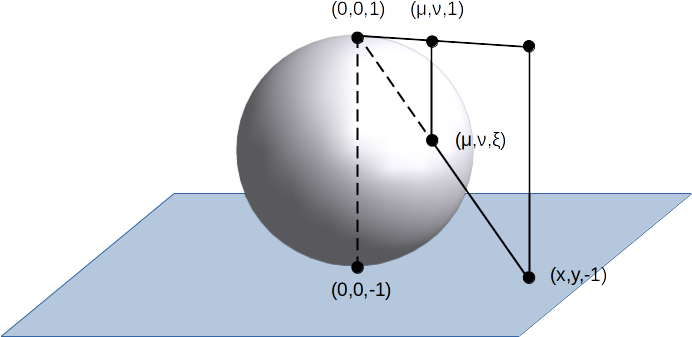
\includegraphics[scale=0.5]{stereo.png}
\end{center}
\caption{Projection stéréographique}
\end{figure}
Pour obtenir un homéomorphisme (i.e. une application bijective continue dont l'inverse est continue) entre $\overline{\C}$ et $\mathbb{S}^2$, il est courant d'avoir recours à une transformation particulière appelée projection stéréographique, qui est également utilisée en géographie pour établir des cartes des régions polaires. Son principe, qui consiste associer de façon univoque un point du plan à un point de la sphère $\mathbb{S}^2$, est résumé en figure \ref{fig:stereo}. Une application immédiate du théorème de Thalès permet d'obtenir les relations suivantes qui définissent la projection:
\begin{equation}
\label{eq:stereo}
x = \frac{2 \mu}{1-\xi} , \, y = \frac{2 \nu}{1-\xi}
\end{equation}
La projection inverse s'obtient tout aussi simplement en utilisant à nouveau Thalès pour obtenir la relation:
\[
x^2 + y^2 = \frac{4}{(1-\xi)^2}\left(\mu^2+\nu^2\right) = \frac{4}{(1-\xi)^2}\left(1-\xi^2\right) = 4 \frac{1+\xi}{1-\xi}
\]
d'où l'on déduit:
\[
\xi = \frac{\left(\frac{r}{2}\right)^2 -1}{\left(\frac{r}{2}\right)^2 +1}, \, r^2 = x^2 + y ^2
\]
puis:
\[
\mu = \frac{x}{\left(\frac{r}{2}\right)^2 +1}, \, \nu = \frac{x}{\left(\frac{r}{2}\right)^2 +1}
\]
En interprétant le plan de projection comme le plan complexe, le point $z = x + i y$ sera transformé en:
\[
\phi(z) = \left(\frac{x}{\left(\frac{|z|}{2}\right)^2 +1}, \frac{y}{\left(\frac{|z|}{2}\right)^2 +1},\frac{\left(\frac{|z|}{2}\right)^2 -1}{\left(\frac{|z|}{2}\right)^2 +1}\right)
\]
En faisant tendre $|z|$ vers $+\infty$ dans l'expression précédente, on remarque que l'on tend vers le point de coordonnées $(0,0,1)$. Ceci permet d'étendre la projection stéréographique inverse à $\overline{\C}$ en posant $\phi(\omega) = (0,0,1)$, établissant ainsi un homéomorphisme entre $\overline{\C}$ et $\mathbb{S}^2$. Du point de vue topologique, ces deux objets sont donc indiscernables. 
\subsection{Connexité}
Intuitivement, une partie connexe est d'un seul tenant: elle ne peut pas être séparée en deux sous-ensembles disjoints à l'aide d'ouverts. Il s'agit d'une notion très fréquemment utilisée dans la théorie des fonctions de la variable complexe. 
\begin{fdefn}
On dira qu'une partie $A$ de $\C$ est connexe s'il n'existe pas deux ouverts $U,V$ de $\C$ tels que $A\cap U \neq \emptyset, A \cap V \neq \emptyset$, $A = (A \cap U) \cup (A \cap V)$ et $(A\cap U)\cap(A \cap V) = \emptyset$.
\end{fdefn}
On montre que cette définition équivaut à la suivante :

\begin{fdefn}
Une partie $A$ de $\C$ est connexe si les seules parties de $A$ à la fois ouvertes et fermées sont $A$ et $\emptyset$
\end{fdefn}

La notion de connexité formalise le fait intuitif d'être d'un seul tenant. Les disques ouverts (resp. fermés) de $\C$ sont des parties connexes. Ceci est la conséquence d'un résultat plus général, donné ci-dessous. 
\begin{fdefn} Un ouvert $U$ de $\C$ est dit \textbf{étoilé} par rapport au point $z_0 \in U$, si pour tout point appartenant à  $U$, le segment de droite joignant $z_0$ à ce point est contenu dans $U$. 
\end{fdefn}


\begin{fprop}
Tout ouvert étoilé de $\C$ est connexe.
\end{fprop}
\begin{proof}
Soit $W$ un ouvert de $\C$ étoilé par rapport au point $z_0$. Supposons qu'il existe deux ouverts $U,V$ tels que $A\cap U \neq \emptyset$, $A \cap V \neq \emptyset$, $U \cap V \cap W = \emptyset$ et $W \subset U \cup V$. Tout point de $W$ appartient donc exclusivement soit à $U$, soit à $V$. Supposons que $z_0 \in U$. Il existe $z_1 \in V \cap W$ et $W$ étant étoilé, le segment: $[z_0,z_1] = \{ (1-t)z_0 + t z_1, \, t \in [0,1]$ appartient à $W$. Soit $\eta = \sup \{ t \in [0,1[ \, \forall u \in [0,t], \,(1-u)z_0 + u z_1 \in U\}$. Si $z_\eta = (1-\eta)z_0 + \eta z_1 \in U$, alors, $U$ étant ouvert, il existe un disque ouvert $D(z_\eta, \epsilon), \epsilon > 0$ inclus dans $U$. Le point $(1-\eta-\epsilon/(2|z_1-z_0|))z_0 + (\eta + \epsilon / (2|z_1-z_0|))z_1$ appartient à $U$, mais aussi à $V$ par définition du $\sup$, ce qui est une contradiction. Le même raisonnement s'applique si $z_\eta \in V$, prouvant ainsi la proposition. 
\end{proof}
La connexité se comporte bien vis-à-vis d'opérations usuelles. En particulier, un produit d'espace connexes est connexe. La proposition suivante est très importante en pratique:
\begin{fprop}
Soit $A$ une partie connexe et $f \colon \C \to \C$ une application continue. Alors la partie $f(A)$ est connexe.
\end{fprop}
\begin{proof}
Supposons l'existence de deux ouverts $U,V$ tels que $f(A)\cap U \neq \emptyset$,$f(A)\cap V \neq \emptyset$, $f(A)\cap U\cap V = \emptyset$ et $f(A) \subset U \cup V$. $f$ étant continue, $f^{-1}(U), f^{-1}(V)$ sont des ouverts tels que: $f^{-1}(U)\cap A \neq \emptyset, f^{-1}(V)\cap A \neq \emptyset$, $f^{-1}(U)\cap f^{-1}(V)\cap A = \emptyset$ et $A \subset f^{-1}(U)\cup f^{-1}(V)$, ce qui est une contradiction, $A$ étant supposée connexe. 
\end{proof}

Enfin, bien que la réunion de parties connexes ne soit généralement pas connexe, ceci est cependant vrai dans le cas où leur intersection n'est pas vide.
\begin{fprop}
\label{prop:union_connexes}
Soit $A_i, i \in I$ une famille quelconque de parties connexes telle que $\bigcap_{i \in I} A _i \neq \emptyset$. Alors $\bigcup_{i \in I} A_i$ est connexe.
\end{fprop}
\begin{proof}
Soient deux ouverts $U,V$ tels que:
\[
U \cap \bigcup_{i \in I} A_i \neq \emptyset, \, V \cap \bigcup_{i \in I} A_i \neq \emptyset, \, U \cap V \cap \bigcup_{i \in I} A_i , \, \bigcup_{i \in I} A_i \subset U \cup V
\]
Soit $x \in \bigcap_{i \in I} A_i$. Par hypothèse $x \in U$ ou $x \in V$. Supposons que $x \in U$ et soit $y \in V \cap \bigcup_{i \in I} A_i $. Il existe $A_k$ tel que: $x \in A_k, \, y \in A_k$. On a donc $U \cap A_k \neq \emptyset, \, V \cap A_k \neq \emptyset$, mais aussi $U \cap V \cap A_k = \emptyset, A_k \subset U \cup V$ ce qui est impossible, $A_k$ étant connexe.
\end{proof}
L'ensemble des parties connexes incluses dans une partie et contenant un point donné vérifie les hypothèses de la proposition précédente. On peut donc parler de plus grande partie connexe contenant un point. Ceci permet d'énoncer le résultat suivant.
\begin{fprop}
Soit $A$ une partie de $\C$. Il existe une partition de $A$ en parties connexes que l'on appelle composantes connexes de $A$.
\end{fprop}
\begin{proof}
Chaque point de $A$ est contenu dans une plus grande partie connexe. En vertu de la proposition \ref{prop:union_connexes}, ces parties sont disjointes car maximales au sens de l'inclusion et forment donc une partition de $A$.
\end{proof}
\begin{rem}
Dans un ouvert $U$ de $\C$, toute composante connexe est ouverte. Soit en effet $x \in U$ et soit $A$ la composante connexe de $U$ le contenant. $U$ étant ouvert, il existe un disque ouvert $D(x,\epsilon)$ contenu dans $U$, mais un disque ouvert étant un ouvert étoilé, il est connexe et est donc inclus dans $A$. On en déduit que $A$ est voisinage de chacun de ses points, donc ouvert.
\end{rem}
\begin{rem}
La remarque précédente montre également que tout ouvert de $\C$ est réunion dénombrable d'ouverts connexes. C'est une conséquence directe de la densité des complexes à coordonnées rationnelles dans $\C$. 
\end{rem}
\subsection{Chemins et connexité par arcs}
\begin{fdefn}
Un chemin de $\C$ est une application continue $\gamma \colon [a,b] \to \C$.
Le point $\gamma(a)$ (resp. $\gamma(b)$) est appelé origine du chemin (resp. extrémité).
\end{fdefn}
\begin{fdefn}
On dira qu'une partie $A$ de $\C$ est connexe par arcs si pour tout couple $(z_0,z_1)$ de points de $A$, il existe un chemin $\gamma \colon [a,b]\to A$ tel que $\gamma(a) = z_0, \gamma(b)=z_1$.
\end{fdefn}
La connexité par arcs est une propriété plus forte que la connexité simple. 
\begin{fprop}
\label{prop:ouvert_connexe}
Toute partie connexe par arcs est connexe et tout ouvert connexe de $\C$ est connexe par arcs. 
\end{fprop}
\begin{proof}
Soit $A$ une partie connexe par arcs et soient $U,V$ deux ouverts de $\C$ tels que $A \cap U \neq \emptyset, A \cap V \neq \emptyset$ et $A \subset U \cup V, A \cap U \cap V = \emptyset$. Soit $z_0 \in U, z_1 \in V$. Par hypothèse, il existe un chemin $\gamma \colon [a,b] \to A$ tel que $\gamma(a) = z_0, \gamma(b)= z_1$. Soit $\eta = \sup \{ t \in [0,1], \gamma([0,t]) \in U\}$. Soit $D(\gamma(\eta),r), r >0$ un disque ouvert contenu dans $U\cup V$. Par continuité de $\gamma$, il existe $\epsilon > 0$ tel que $\gamma(]\eta-\epsilon, \eta +\epsilon[) \subset D(\gamma(\eta),r)$. $D(\gamma(\eta),r)\cap U \neq \emptyset$ car $\gamma([0,t]) \in U$ si $t < \eta$ et $D(\eta,r) \cap V \neq \emptyset$ car par définition du $\sup$, il existe des points de $V$ appartenant à $\gamma([\eta,\eta + \epsilon/2])$. Or $\eta \in U$ ou $\eta \in V$ et $U,V$ sont des ouverts, il devrait donc exister un rayon $r^\prime > 0$ tel que $D(\gamma(\eta),r^\prime)\subset U$ ou $D(\gamma(\eta),r^\prime)\subset V$, ce qui est contradictoire. 

La seconde partie de la proposition, que l'on peut voir comme une réciproque partielle, utilise un très important argument basé sur la connexité simple que l'on retrouvera un peu plus loin dans le cours. Soit $U$ un ouvert connexe de $\C$ et $z_0$ un point de $U$. L'ensemble $A=\{ z \in U , \, \exists \gamma \colon [a,b] \to U, \gamma(a)=z_0, \gamma(b) = z\}$ est un ouvert. En effet, soit $z \in A$. $U$ étant ouvert, il existe $D(z, \epsilon), \epsilon > 0$ tel que $D(z,\epsilon) \subset U$. Soit $u \in D(z,\epsilon)$. Par hypothèse, il existe un chemin $\gamma$ d'origine $z_0$ et d'extrémité $z$. D'autre par, le segment $[z,u]$ appartient à $D(z, \epsilon)$, donc à $U$ et le chemin obtenu concaténant $\gamma$ avec $[z,u]$ est continu, d'où $u \in A$. $U-A$ est également un ouvert. En effet, soit $z \in U-A$.Il existe $\epsilon > 0$ tel que $D(z,\epsilon) \subset U$. $D(z,\epsilon)$ ne peut contenir aucun point de $A$ sans quoi il existerait un chemin joignant $z_0$ à $z$. On a donc $D(z,\epsilon) \subset U-A$. Les ouverts $A,U-A$ sont disjoints, d'union $U$. Comme $A$ n'est pas vide car contenant au moins $z_0$, on doit avoir $U-A=\emptyset$ par connexité de $U$, ce qui termine la démonstration.
\end{proof}
La connexité par arcs est préservée par les applications continues.
\begin{fprop}
Soit $A \subset \C$ une partie connexe par arcs et $f \colon \C \to \C$ une application continue. Alors $f(A)$ est connexe par arcs.
\end{fprop}
\begin{proof}
Soient $z_0,z_1 \in f(A)$. Il existe $p,q \in A$ tels que $f(p) =z_0, f(q)=z_1$. $A$ étant connexe par arcs, il existe $\gamma \colon [a,b] \to A$ tel que $\gamma(a) = p, \gamma(b) = q$. L'application $f \circ \gamma$ est un chemin reliant $z_0,z_1$, prouvant ainsi la connexité par arcs de $f(A)$.
\end{proof}
\begin{exercice}
    Montrer que $\C$ et $\R$ ne sont pas homéomorphes. 
    
    \textbf{Indication:} Montrer que si $\phi \colon \C \to \R$ est un homéomorphisme, alors $\Phi\left(\C-\{0\}\right)$ n'est pas connexe.    
\end{exercice}
\begin{fdefn} Un sous ensemble $\Omega$ du plan complexe est un \textbf{domaine} si $\Omega$ est un ouvert non vide connexe. 
\end{fdefn}
\begin{rem}
En vertu de la proposition \ref{prop:ouvert_connexe}, il équivalent de vérifier que $\Omega$ est connexe par arcs, ce qui est souvent plus simple.
\end{rem}

Un disque ouvert de rayon non nul est un domaine, de même qu'une couronne ouverte définie comme:
\[
\mathcal{C}(z;r_1,r2) =  \{ z : 0<r_1 <\lvert z-z_0 \rvert <r_2\}. 
 \]
 Tout ouvert étoilé non vide est un domaine.


\begin{figure}[H]
\begin{center}
\shorthandoff{!}\shorthandoff{:}

\begin{tikzpicture}
\clip(-3,-3) rectangle (10,3);
\begin{scope}[xshift=7 cm]
 \tikzstyle{point}=[circle,thick,draw=black,fill=black,inner sep=0pt,minimum width=4pt,minimum height=4pt]
    \fill[color=gray!40] (-2,0) -- (-1,0.5) -- (0,2) -- (1,0.5) -- (2,0) -- (1,-0.5) -- (0,-2) -- (-1,-0.5) -- cycle;
    \node (a)[point,label=$z_0$] at (0,0) {};
\end{scope}
\fill[color=gray!40,even odd rule] (0,0) circle(1) circle(2);
\end{tikzpicture}
\shorthandon{!}\shorthandoff{:}
\caption{Exemples de domaines : anneau et ouvert étoilé par rapport à $z_0$. Notons que l'anneau n'est étoilé par rapport à aucun de ses points.}\label{fig:domaines}
\end{center}
\end{figure}
 Dans la suite, nous désignerons par $U$ les ouverts de $\C$ et par $\Omega$ les domaines de $\C$. Les domaines joueront un rôle important dans la théorie de l'intégration d'une fonction de la variable complexe le long d'un chemin.



\begin{fdefn}
Soit $U$ un ouvert de $\C$. Un chemin de classe $C^k$ par morceaux dans $U$ est une application continue $\gamma$ d'un intervalle réel $[a,b]$ dans $U$ telle qu'il existe une subdivision $a=t_0 < t_1 < \dots < t_N = b$ pour laquelle $\gamma$ est de classe $C^k$ sur chaque intervalle $]t_i,t_{i+1}[, \, i=0 \dots N$. Nous dirons que $\gamma$ est un chemin joignant les points $\gamma(a)$ (l'origine) et $\gamma(b)$ (l'extrémité) dans $U$.
\end{fdefn}
Dans toute la suite, le terme \og chemin \fg{} désignera de façon implicite un chemin de classe $C^k$ par morceaux, l'indice de régularité $k$ étant précisé lorsque cela est nécessaire. 

L'ensemble image $\lvert\gamma \rvert:=\gamma([a, b])\subset U$ est appelé \emph{trace} du chemin. Comme $\gamma$ est continue, $\lvert\gamma \rvert$ est un ensemble compact. Il convient de noter qu'un chemin est plus que sa simple trace ; cette dernière étant traversée selon la loi $\gamma(t)$. En particulier :

\begin{fdefn}
Soit $\gamma \colon [a,b] \to U$ un chemin. Soit $\phi \colon [c,d] \to [a,b]$ un difféomorphisme de classe $C^k$. Le chemin $\gamma \circ \phi$ sera dit obtenu à partir de $\gamma$ par changement de paramètre. Un changement de paramètre $\phi$ strictement croissant sera dit préservant l'orientation.
\end{fdefn}
La trace d'un chemin obtenu par changement de paramètre est semblable à celle du chemin initial. Son sens de parcours n'est pas modifié si le changement de paramètre préserve l'orientation. Dans toute la suite, les grandeurs associées aux chemins seront invariantes par changement de paramètre préservant l'orientation: on pourra donc choisir de façon arbitraire l'intervalle de définition d'un chemin de telle sorte que les calculs soient les plus simples possible. Pour les définitions qui vont suivre, on se placera sur l'intervalle $[0,1]$ afin d'alléger les écritures. Nous utiliserons également la notation $\gamma$ pour définir le chemin et sa trace.


\begin{exem}
\begin{enumerate}
\item Un chemin $\gamma$ est appelé chemin \textbf{nul}, si la fonction $\gamma$ est constante. La trace est alors constituée d'un seul point. Un tel chemin est continument différentiable.
\item Le segment $[z_0, z_1]$ est le chemin continument différentiable défini par
\[\gamma(t) := (1 - t)z_0 + tz_l, \quad t \in [0,1].\]
\item Soit $c \in \C$, et $r > 0$. La fonction 
\[\gamma(t) := c + r e^{it}, \quad t \in [a,b],\]
avec $0 \leq a < b \leq 2 \pi$ est continument différentiable. Le chemin $\gamma$ correspondant est un arc circulaire situé sur la frontière du disque $B(c;r)$. Lorsque $a=0$ et $b=2 \pi$, le chemin $\gamma$ est le cercle centré en $c$ et de rayon $r$.  
\end{enumerate}
\end{exem}



\begin{fdefn}
Un chemin $\gamma$ est dit \textbf{simple} si $\gamma(s) \neq \gamma(t)$ quand $s\neq t$. Un chemin est appelé \textbf{lacet} si son origine coïncide avec son extrémité, donc si $\gamma(0)=\gamma(1)$. Un \textbf{lacet simple} est un lacet tel que $ \gamma(s)\neq \gamma(t)$ pour $0 \leq s<t<1$. 
\end{fdefn}


\begin{figure}[H]
\begin{center}
\shorthandoff{!}\shorthandoff{:}
\begin{tikzpicture}
\tikzset{
    on each segment/.style={
        decorate,
        decoration={
            show path construction,
            moveto code={},
            lineto code={
                \path [#1]
                (\tikzinputsegmentfirst) -- (\tikzinputsegmentlast);
            },
            curveto code={
                \path [#1] (\tikzinputsegmentfirst)
                .. controls
                (\tikzinputsegmentsupporta) and (\tikzinputsegmentsupportb)
                ..
                (\tikzinputsegmentlast);
            },
            closepath code={
                \path [#1]
                (\tikzinputsegmentfirst) -- (\tikzinputsegmentlast);
            },
        },
    },
}
    \begin{scope}[scale=2]
        \node[label=below:$A$] (A) at (0,0) {};
        \node[label=below:$B$] (B) at (2,0.25){};
        \draw[blue] plot [smooth,tension=1]
        coordinates {(A) (1,0) (1.14,-0.6) (0.5,-0.5) (0.5,0.5) (1.5,0) (B)}[postaction={on each segment={draw,-{stealth[red,bend]}}}];
        \draw (1, -1) node {chemin quelconque};
        \draw [fill=black] (A) circle (1pt);
    \draw [fill=black] (B) circle (1pt);
    \end{scope}
    \begin{scope}[scale=2,xshift= 3 cm]
        \node[label=below:$A$] (A) at (0,0) {};
        \node[label=below:$B$] (B) at (2,0.25){};
        \draw[blue] plot [smooth,tension=1]
        coordinates {(A)  (0.5,0.5) (1.5,0) (B)}[postaction={on each segment={draw,-{stealth[red,bend]}}}];
        \draw (1, -1) node {chemin simple};
        \draw [fill=black] (A) circle (1pt);
    \draw [fill=black] (B) circle (1pt);
    \end{scope}
\begin{scope}[scale=2,xshift= 6 cm]
        \node[label=below:$A$] (A) at (0,0) {};
       % \node[label=below:$B$] (B) at (2,0.25){};
        \draw[blue] plot [smooth,tension=1]
        coordinates {(A)  (0.5,0.5) (1.5,0.25) (1.5,-0.25) (0.5,-0.5) (A)}[postaction={on each segment={draw,-{stealth[red,bend]}}}];
        \draw (1, -1) node {lacet simple};
        \draw [fill=black] (A) circle (1pt);
   
    \end{scope}    
    
    
\end{tikzpicture}

\shorthandon{!}\shorthandoff{:}

\end{center}
\end{figure}



\begin{fdefn}
Soient $\gamma_1, \gamma_2$ deux chemins de $[0,1]$ dans un ouvert $U$ de $\C$ tels que $\gamma_1(1) =
\gamma_2(0)$. Le chemin $\gamma_2 + \gamma_1$, somme de $\gamma_1$ et
$\gamma_2$, est défini par :
\[(\gamma_2 + \gamma_1)(t) = \left \{
\begin{array}{cc}
\gamma_1(2t) & \text{ si } t \in \left[0,\frac{1}{2}\right] \\
\gamma_2(2t-1) & \text{ si } t \in \left]\frac{1}{2},1\right]
\end{array}
\right.
\]
\end{fdefn}

Le chemin $\gamma_1 + \gamma_2 + \cdots + \gamma_n$ somme d'un nombre fini des chemins $\gamma_1,\gamma_2,\cdots, \gamma_n$ (dont les origines et extrémités sont appropriées) est défini de la même façon. On vérifie que la somme des chemins est une opération associative, elle n'est pas commutative. Notons qu'il est toujours possible d'écrire de décomposer un chemin $C^k$ par morceaux en une somme de chemins $C^k$. 


\begin{fdefn}
Soit $\gamma$ un chemin de $[0,1]$ dans un ouvert $U$ de $\C$. Le chemin opposé, noté
$-\gamma$, est défini par:
\[(-\gamma)(t) = \gamma(1-t), \quad t \in [0,1]
\]
\end{fdefn}
Le chemin opposé est obtenu par le changement de paramètre $\phi(t)=1-t$ qui ne préserve pas l'orientation. Le chemin opposé possède donc la même image, mais est \og parcouru dans la direction opposée \fg{}.
Les opérations sur les chemins sont résumées figure \ref{ch8:fig1}.
%\begin{figure}[ht]
%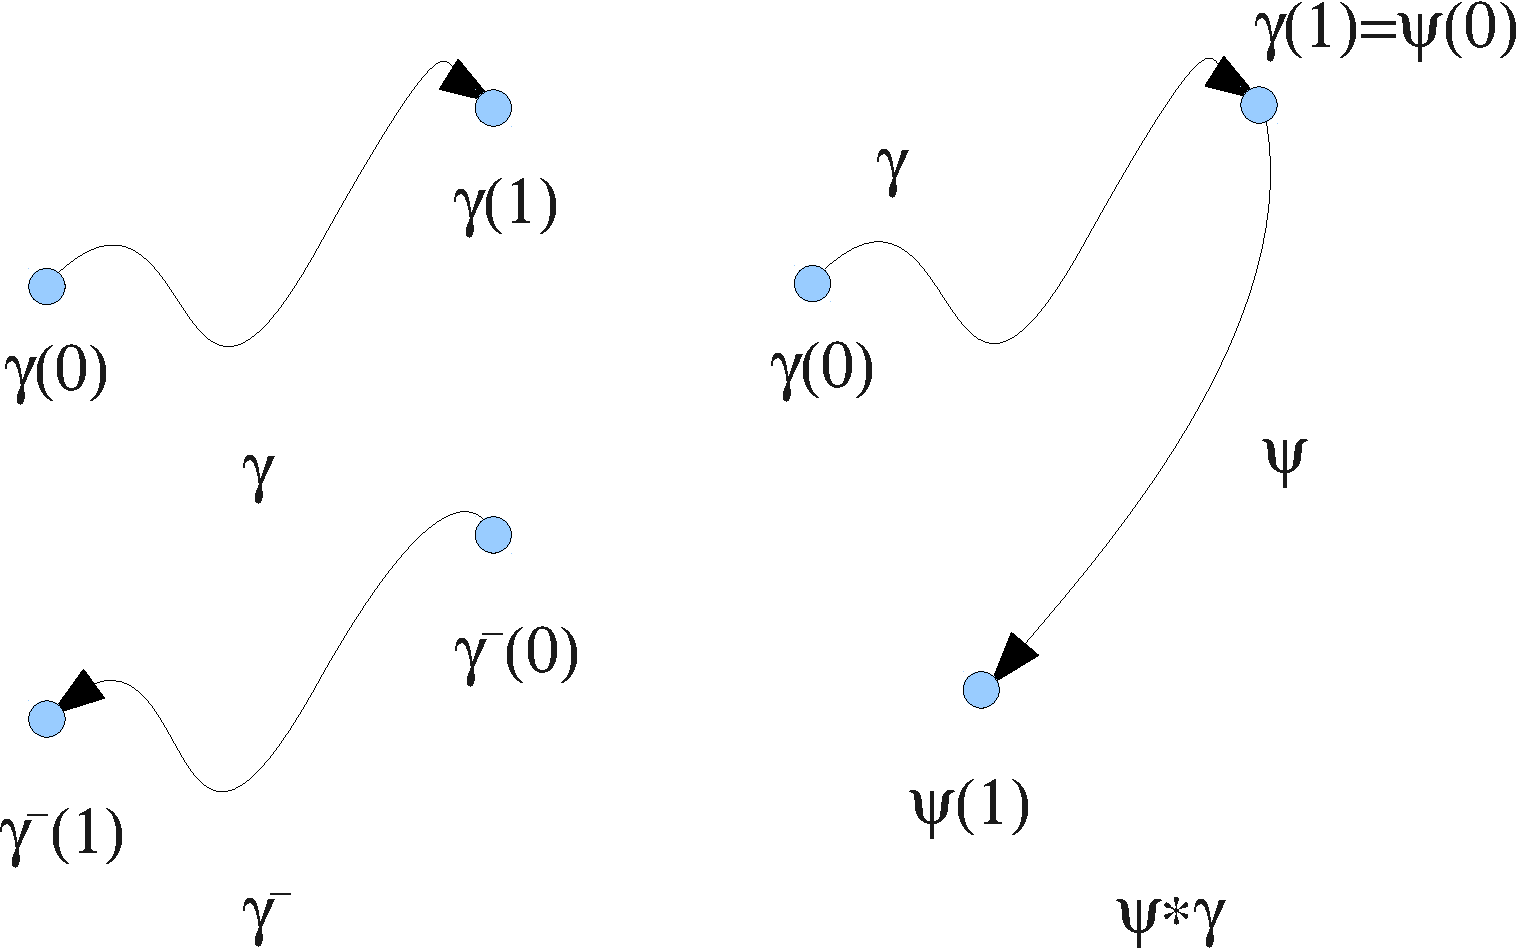
\includegraphics[scale=0.4]{images/chemins.pdf}
%\caption{Chemins composé et inverse}\label{ch8:fig1}
%\end{figure}
\begin{figure}[ht]
\begin{center}
\shorthandoff{!}\shorthandoff{:}
\begin{tikzpicture}
\tikzset{
    on each segment/.style={
        decorate,
        decoration={
            show path construction,
            moveto code={},
            lineto code={
                \path [#1]
                (\tikzinputsegmentfirst) -- (\tikzinputsegmentlast);
            },
            curveto code={
                \path [#1] (\tikzinputsegmentfirst)
                .. controls
                (\tikzinputsegmentsupporta) and (\tikzinputsegmentsupportb)
                ..
                (\tikzinputsegmentlast);
            },
            closepath code={
                \path [#1]
                (\tikzinputsegmentfirst) -- (\tikzinputsegmentlast);
            },
        },
    },
}
    
     
    
  \begin{scope}[scale=2]
        \node[label=below:$\gamma(0)$] (A) at (0,0) {};
        \node[label=above:$\gamma(1)$] (B) at (2,0.25){};
        \draw[blue] plot [smooth,tension=1]
        coordinates {(A)  (0.5,0.5) (1.5,0) (B)}[postaction={on each segment={draw,-{stealth[red,bend]}}}];
       \draw [fill=black] (A) circle (1pt);
    \draw [fill=black] (B) circle (1pt);
  \end{scope}    
    
  \begin{scope}[scale=2, yshift=-1cm]     
      \node[label=below:$-\gamma(1)$] (A) at (0,0) {};
        \node[label=above:$-\gamma(0)$] (B) at (2,0.25){};
        \draw[blue] plot [smooth,tension=1]  
    coordinates {(B)  (1.5,0) (0.5,0.5)  (A)}[postaction={on each segment={draw,-{stealth[red,bend]}}}];
       \draw [fill=black] (A) circle (1pt);
    \draw [fill=black] (B) circle (1pt);    
    \end{scope}
  
  \begin{scope}[scale=2, xshift = 3cm]
        \node[label=below:$\gamma_1(0)$] (A) at (0,0) {};
        \node[label=above:{$\gamma_1(1)=\gamma_2(0)$}] (B) at (2,0.25){};
        \draw[blue] plot [smooth,tension=1]
        coordinates {(A)  (0.5,0.5) (1.5,0) (B)}[postaction={on each segment={draw,-{stealth[red,bend]}}}];
       \draw [fill=black] (A) circle (1pt);
    \draw [fill=black] (B) circle (1pt);
       \node[label=below:$\gamma_2(1)$] (C) at (3.5,0.25){};
        \draw[blue] plot [smooth,tension=1]
       coordinates {(B)  (2.5,-0.5) (3,0) (C)}[postaction={on each segment={draw,-{stealth[red,bend]}}}];
      \draw [fill=black] (C) circle (1pt);
   \end{scope}     
    
        
\end{tikzpicture}

\shorthandon{!}\shorthandoff{:}
\caption{Chemins inverse et composé.}\label{ch8:fig1}
\end{center}
\end{figure}


Il est possible de définir la longueur d'un chemin en l'approchant par des chemins polygonaux: c'est Archimède qui semble-t-il est le premier à avoir eu cette idée. La proposition suivante résume ce procédé.
\begin{fprop}
Soit $\gamma \colon [a,b] \to \C$ un chemin de classe $C^k$, $k \geq 1$. Pour toute subdivision $\mathcal{S} = \{a=t_0 < t_1 \dots < t_n = b\}$ de l'intervalle $[a,b]$, on pose :
\[
l(\mathcal{S}) = \sum_{i=0}^{n-1} \lvert \gamma(t_{i+1}) - \gamma(t_i) \rvert.
\]
La borne supérieure de l'ensemble $\{l(\mathcal{S})\}$ où $\mathcal{S}$ parcourt les subdivisions de $[a,b]$ est finie et vaut :
\[
l(\gamma) = \int_a^b \lvert\gamma^\prime(t)\rvert \diff t.
\]
la valeur $l(\gamma)$ est appelée longueur du chemin $\gamma$.
\end{fprop}
\begin{proof}
On remarque tout d'abord, en vertu du théorème des accroissements finis que :
\[
\lvert \gamma(t_{i+1}) - \gamma(t_i) \rvert  = \left\lvert \int_{t_i}^{t_{i+1}} \gamma^\prime(s) \diff s \right\rvert \leq \int_{t_i}^{t_{i+1}}\left\lvert \gamma^\prime(s) \right\rvert\diff s .\]
On en déduit que pour toute subdivision $\mathcal{S}$ :
\[
l(\mathcal{S}) \leq  \int_a^b \left\lvert \gamma^\prime(s) \right\rvert \diff s,\]
et par conséquent la borne supérieure de l'ensemble $\{l(\mathcal{S})\}$ où $\mathcal{S}$ parcourt les subdivisions de $[a,b]$ est donc finie. Soit maintenant $\epsilon > 0$, l'application $\gamma$ étant de classe $C^1$, sa dérivée est continue sur le compact $[a,b]$, donc uniformément continue. Il existe donc $\eta>0$, telle que pour toute subdivision $\mathcal{S} = \{a=t_0 < t_1 \dots < t_n = b\}$  dont le pas, $\delta :=\sup_{i=0}^{n-1}(t_{i+1}-t_i)$, est tel que $\delta<\eta$, on ait, pour tout $i=0, \cdots, n-1$, l'inégalité 
\[
\lvert \gamma^\prime(s) - \gamma^\prime(t_i)\rvert < \epsilon, \quad s \in [t_i, t_{i+1}].
\]
Ceci implique que pour tout $i=0,\dots,n-1$:
\begin{align*}
\Bigl \lvert\int_{t_i}^{t_{i+1}} (\gamma^\prime(s) - \gamma^\prime(t_i)) \diff s \Bigr \rvert & = \lvert \gamma(t_{i+1}) - \gamma(t_i) - \gamma^\prime(t_i) (t_{i+1}- t_i) \rvert \\& < \epsilon (t_{i+1}-t_i),
\end{align*}
soit finalement :
\[
\Bigl \lvert \lvert\gamma(t_{i+1}) - \gamma(t_i)\rvert -  \lvert\gamma^\prime(t_i) \rvert(t_{i+1}-t_i)\Bigr \rvert < \epsilon (t_{i+1}-t_i).
\]
On en déduit par sommation sur $i$ et application de l'inégalité triangulaire :
\[
\Bigl \lvert l(S) - \sum_{i=0}^n  \lvert\gamma^\prime(t_i) \rvert(t_{i+1}-t_i)\Bigr \rvert < \epsilon (b-a).
\]
Par une propriété connue des intégrales de Riemann, il existe un $\eta^\prime$ tel que si $\delta< \eta^\prime$, alors :  
\[
\Bigl  \lvert \int_a^b \lvert\gamma^\prime(s)\rvert ds -  \sum_{i=0}^n  \lvert\gamma^\prime(t_i) \rvert(t_{i+1}-t_i) \Bigr \rvert  < \epsilon .\]
En choisissant $\eta_0=\min (\eta, \eta^\prime)$, pour toute subdivision de pas $\delta<\eta_0$, 
\[ \Bigl \lvert l(\mathcal{S}) - \int_a^b \lvert\gamma^\prime(s)\rvert \diff s \Bigr \rvert < \epsilon(1 + (b-a)),\]
ce qui termine la preuve.
\end{proof}
Lorsque le chemin est de classe $C^k$ par morceaux, on définit sa longueur par sommation. 
\begin{fdefn}
Soit $\gamma \colon [a,b] \to \C$ un chemin de classe $C^k$ sur chacun des intervalles $]t_i,t_{i+1}[$, où $\{a=t_0 < t_1 \dots < t_n = b\})$ est une subdivision de l'intervalle $[a,b]$. Sa longueur est définie par:
\[
l(\gamma) = \sum_{i=0}^{n-1} \int_{t_i}^{t_{i+1}} \lvert \gamma^\prime(t) \rvert \diff t
\]
\end{fdefn}
La proposition suivante établit le fait que la longueur d'un chemin est un invariant géométrique qui ne dépend que de sa trace et non de sa paramétrisation. Cette proposition se prouve en utilisant la formule du changement de variable dans les intégrales. 
\begin{fprop}
La longueur d'un chemin de classe $C^k$ par morceaux est invariante par changement de paramétrage.
\end{fprop}
\begin{rem}
Le procédé d'approximation par des chemins polygonaux permet de définir la longueur de chemins simplement continus, mais celle-ci peut être infinie. C'est par exemple le cas de courbe fractale comme la courbe de Koch. Cette dernière s'obtient à partir d'un segment de droite en modifiant récursivement chaque segment de droite de la façon suivante : 
1) on divise le segment de droite en trois segments de longueurs égales, 2) on construit un triangle équilatéral ayant pour base le segment médian de la première étape, 3) on supprime la base du triangle de la deuxième étape (cf. figure~\ref{fig:Koch}). On peut montrer qu'à l'étape $n$, la longueur de la courbe obtenue est supérieure à $(4/3)^n$. Lorsque la longueur d'un chemin est finie, on dit que le chemin est \textbf{rectifiable}. L'absence de formule de calcul utilisable dans le cas général fait qu'en pratique, on se restreint aux chemins de classe $C^k$ par morceaux.
\begin{figure}[ht]
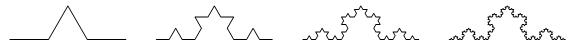
\includegraphics[scale=0.8]{courbe_Koch}
\caption{Courbe de Von Koch : les quatre premières étapes}\label{fig:Koch}
\end{figure}
 
\end{rem}
\section{Exercice complémentaire}
\begin{exer}[\textbf{Projection stéréographique}]
Le but de cet exercice est d'établir une formule explicite connectant le point $z = x +i y \in \C$ et sa projection $\hat{z}$ sur $\Sigma$. Soit $(X,Y,Z)$ les coordonnées cartésiennes de $\hat{z}$, où l'axe $Z$ passe par $N$ et les axes $X$ et $Y$ coïncident avec les axes $x,y$ de $\C$.  Soit $z' = X+i Y$ le pied de la perpendiculaire à $\C$ passant par $\hat{z}$. 

\begin{figure}[ht]
\begin{center}
\shorthandoff{!}\shorthandoff{:}
\begin{tikzpicture}[line cap=round,line join=round,>=triangle 45,x=9.999999999999998cm,y=10.0cm, scale=0.3]
\clip(-1.0204444716563346,-1.1991274885913612) rectangle (2.500817665540407,1.2986943169702587);
\draw[fill opacity=0.10000000149011612] (0.055454528631341884,0.6249841873023777) -- (0.05545452863134189,0.6804387159337196) -- (0.,0.6804387159337196) -- (0.,0.6249841873023777) -- cycle; 
\draw[fill opacity=0.10000000149011612] (0.055454528631341884,0.) -- (0.05545452863134189,0.05545452863134188) -- (0.,0.055454528631341884) -- (0.,0.) -- cycle; 
\draw[fill opacity=0.10000000149011612] (0.8360919384587128,0.) -- (0.8360919384587128,0.05545452863134188) -- (0.7806374098273708,0.055454528631341884) -- (0.7806374098273708,0.) -- cycle; 
\draw(0.,0.) circle (10.cm);
\draw (0.,1.)-- (2.081611983804011,0.);
\draw (0.,0.)-- (0.7806374098273708,0.6249841873023777);
\draw (0.5519676853769542,-0.8697443933524662) node[anchor=north west] {$\Sigma$};
\draw (-0.09895605045228752,-0.010995609336775847) node[anchor=north west] {$O$};
\draw (-0.11464095974937767,1.1849787245663546) node[anchor=north west] {$N$};
\draw (0.8225323707517594,0.7850135374905536) node[anchor=north west] {$\hat{z}$};
\draw (2.0930100238160625,0.13016857433703627) node[anchor=north west] {$z$};
\draw [line width=0.4pt] (0.,0.6249841873023777)-- (0.7806374098273708,0.6249841873023777);
\draw [line width=0.4pt] (0.7806374098273708,0.6249841873023777)-- (0.7806374098273708,0.);
\draw (0.7558715062391264,-0.003153154688230729) node[anchor=north west] {$z'$};
\draw (0.573525732429403,0.38112712309048) node[anchor=north west] {$Z$};
\draw (-0.14993200566783055,0.5732672619798354) node[anchor=north west] {$1$};
\draw [domain=-1.0204444716563346:2.500817665540407] plot(\x,{(-0.-0.*\x)/-2.081611983804011});
\draw (0.,1.)-- (0.,0.);
\begin{scriptsize}
\fill [color=pblue] (0.,0.) circle (5pt);
\fill [color=pblue] (0.,1.) circle (5pt);
\fill [color=pblue] (0.7806374098273708,0.6249841873023777) circle (5pt);
\fill [color=pblue] (2.081611983804011,0.) circle (5pt);
\fill [fill=pblue] (0.,0.6249841873023777) circle (5pt);
\fill [color=pblue] (0.7806374098273708,0.) circle (5pt);
\end{scriptsize}
\end{tikzpicture}

\shorthandon{!}\shorthandoff{:}
\caption{Projection stéréographique}\label{fig8}
\end{center}
\end{figure}

Alors $z'$ et $z$ sont dans la même direction, ainsi
\[z=\frac{\lvert z \rvert}{\lvert z' \rvert} z'.\]
\begin{MYenumerate}
\item En observant la figure~\ref{fig8}, qui représente la section verticale de la sphère et de $\C$ passant par $N$ et $\hat{z}$, que les triangles rectangles d'hypoténuse $N \hat{z}$ et $Nz$ sont semblables, en déduire que 
\[\frac{\lvert z \rvert}{\lvert z' \rvert} = \frac{1}{1-Z}.\]
\item Obtenir la première formule
\[x+iy = \frac{X+i Y}{1-Z},\]
puis l'inverser pour trouver les coordonnées de $\hat{z}$ en fonction des coordonnées de $z$.
\item Une cercle sur $\Sigma$ passant par le point $N=(0,0,1)$ est l'intersection du plan d'équation $a X + b Y +c(Z-1)=0$ avec $\Sigma$. En déduire que les images $z$ vérifient une équation de la forme
\[\bar{\alpha} z + \alpha \bar{z}=k \]
avec $\alpha  \in \C^\ast$ et $k \in \R$ que l'on exprimera en fonction des constantes réelles $a,b,c$. Montrer que l'on obtient l'équation d'une droite dans $\C$.
\item Si le cercle ne passe pas par $N$, en raison de la symétrie de la sphère, une simple rotation permet de considérer le cercle comme l'intersection du plan $Z=k$ avec $\Sigma$ (avec $k>0$). Montrer alors que $\lvert z\rvert ^2$ est constant et donc que l'image est un cercle centré à l'origine.  
\end{MYenumerate}
Il existe des démonstrations purement géométriques de ces résultats, par exemple dans l'excellent livre \cite{hilbert1983geometry}.
\end{exer}